%==============================================================================
% tento soubor pouzijte jako zaklad
% this file should be used as a base for the thesis
% Autoři / Authors: 2008 Michal Bidlo, 2016 Jaroslav Dytrych
% Kontakt pro dotazy a připomínky: dytrych@fit.vutbr.cz
% Contact for questions and comments: dytrych@fit.vutbr.cz
%==============================================================================
% kodovaní: UTF-8 (zmena prikazem iconv, recode nebo cstocs)
% encoding: UTF-8 (you can change it by command iconv, recode or cstocs)
%------------------------------------------------------------------------------
% zpracování / processing: make, make pdf, make clean
%==============================================================================
% Soubory, které je nutné upravit: / Files which have to be edited:
%   projekt-20-literatura-bibliography.bib - literatura / bibliography
%   projekt-01-kapitoly-chapters.tex - obsah práce / the thesis content
%   projekt-30-prilohy-appendices.tex - přílohy / appendices
%==============================================================================
\documentclass[]{fitthesis} % bez zadání - pro začátek práce, aby nebyl problém s překladem
%\documentclass[english]{fitthesis} % without assignment - for the work start to avoid compilation problem
%\documentclass[zadani]{fitthesis} % odevzdani do wisu - odkazy jsou barevné
%\documentclass[english,zadani]{fitthesis} % for submission to the IS FIT - links are color
%\documentclass[zadani,print]{fitthesis} % pro tisk - odkazy jsou černé
%\documentclass[zadani,cprint]{fitthesis} % pro barevný tisk - odkazy jsou černé, znak VUT barevný
%\documentclass[english,zadani,print]{fitthesis} % for the color print - links are black
%\documentclass[english,zadani,cprint]{fitthesis} % for the print - links are black, logo is color
% * Je-li prace psana v anglickem jazyce, je zapotrebi u tridy pouzit
%   parametr english nasledovne:
%   If thesis is written in english, it is necessary to use
%   parameter english as follows:
%      \documentclass[english]{fitthesis}
% * Je-li prace psana ve slovenskem jazyce, je zapotrebi u tridy pouzit
%   parametr slovak nasledovne:
%      \documentclass[slovak]{fitthesis}

% Základní balíčky jsou dole v souboru šablony fitthesis.cls
% Basic packages are at the bottom of template file fitthesis.cls
%zde muzeme vlozit vlastni balicky / you can place own packages here

\usepackage{subcaption}
\usepackage{pgfplots}
\usepackage{booktabs}


% tmpframe od herouta http://www.herout.net/blog/2017/03/pomalu-uz-pojdme-psat/
% na konci odkomentovat, slouzi k viditelnemu oramovani obrazku
\setlength{\fboxsep}{0.005pt}
\newcommand{\tmpframe}[1]{\fbox{#1}}
% \renewcommand{\tmpframe}[1]{#1}

%---rm---------------
\renewcommand{\rmdefault}{lmr}%zavede Latin Modern Roman jako rm / set Latin Modern Roman as rm
%---sf---------------
\renewcommand{\sfdefault}{qhv}%zavede TeX Gyre Heros jako sf
%---tt------------
\renewcommand{\ttdefault}{lmtt}% zavede Latin Modern tt jako tt

% vypne funkci šablony, která automaticky nahrazuje uvozovky,
% aby nebyly prováděny nevhodné náhrady v popisech API apod.
% disables function of the template which replaces quotation marks
% to avoid unnecessary replacements in the API descriptions etc.
\csdoublequotesoff

% =======================================================================
% balíček "hyperref" vytváří klikací odkazy v pdf, pokud tedy použijeme pdflatex
% problém je, že balíček hyperref musí být uveden jako poslední, takže nemůže
% být v šabloně
% "hyperref" package create clickable links in pdf if you are using pdflatex.
% Problem is that this package have to be introduced as the last one so it
% can not be placed in the template file.
\ifWis
\ifx\pdfoutput\undefined % nejedeme pod pdflatexem / we are not using pdflatex
\else
  \usepackage{color}
  \usepackage[unicode,colorlinks,hyperindex,plainpages=false,pdftex]{hyperref}
  \definecolor{links}{rgb}{0.4,0.5,0}
  \definecolor{anchors}{rgb}{1,0,0}
  \def\AnchorColor{anchors}
  \def\LinkColor{links}
  \def\pdfBorderAttrs{/Border [0 0 0] }  % bez okrajů kolem odkazů / without margins around links
  \pdfcompresslevel=9
\fi
\else % pro tisk budou odkazy, na které se dá klikat, černé / for the print clickable links will be black
\ifx\pdfoutput\undefined % nejedeme pod pdflatexem / we are not using pdflatex
\else
  \usepackage{color}
  \usepackage[unicode,colorlinks,hyperindex,plainpages=false,pdftex,urlcolor=black,linkcolor=black,citecolor=black]{hyperref}
  \definecolor{links}{rgb}{0,0,0}
  \definecolor{anchors}{rgb}{0,0,0}
  \def\AnchorColor{anchors}
  \def\LinkColor{links}
  \def\pdfBorderAttrs{/Border [0 0 0] } % bez okrajů kolem odkazů / without margins around links
  \pdfcompresslevel=9
\fi
\fi
% Řešení problému, kdy klikací odkazy na obrázky vedou za obrázek
% This solves the problems with links which leads after the picture
\usepackage[all]{hypcap}

% Informace o práci/projektu / Information about the thesis
%---------------------------------------------------------------------------
\projectinfo{
  %Prace / Thesis
  project=DP,            %typ prace BP/SP/DP/DR  / thesis type (SP = term project)
  year=2018,             %rok odevzdání / year of submission
  date=\today,           %datum odevzdani / submission date
  %Nazev prace / thesis title
  title.cs={Strojový překlad pomocí umělých neuronových sítí},  %nazev prace v cestine ci slovenstine (dle zadani) / thesis title in czech language (according to assignment)
  title.en={Machine Translation Using Artificial Neural Networks}, %nazev prace v anglictine / thesis title in english
  %Autor / Author
  author={Jonáš Holcner},   %cele jmeno a prijmeni autora / full name and surname of the author
  author.name={Jonáš},   %jmeno autora (pro citaci) / author name (for reference)
  author.surname={Holcner},   %prijmeni autora (pro citaci) / author surname (for reference)
  author.title.p=Bc., %titul pred jmenem (nepovinne) / title before the name (optional)
  %author.title.a=PhD, %titul za jmenem (nepovinne) / title after the name (optional)
  %Ustav / Department
  department=UPGM, % doplnte prislusnou zkratku dle ustavu na zadani: UPSY/UIFS/UITS/UPGM
  %                  fill in appropriate abbreviation of the department according to assignment: UPSY/UIFS/UITS/UPGM
  %Skolitel / supervisor
  supervisor=Igor Szőke, %cele jmeno a prijmeni skolitele / full name and surname of the supervisor
  supervisor.name={Igor},   %jmeno skolitele (pro citaci) / supervisor name (for reference)
  supervisor.surname={Szöke},   %prijmeni skolitele (pro citaci) / supervisor surname (for reference)
  supervisor.title.p=Ing.,   %titul pred jmenem (nepovinne) / title before the name (optional)
  supervisor.title.a={Ph.D.},    %titul za jmenem (nepovinne) / title after the name (optional)
  %Klicova slova, abstrakty, prohlaseni a podekovani je mozne definovat
  %bud pomoci nasledujicich parametru nebo pomoci vyhrazenych maker (viz dale)
  %Keywords, abstracts, declaration and acknowledgement can be defined by following
  %parameters or using dedicated macros (see below)
  %===========================================================================
  %Klicova slova / keywords
  %keywords.cs={Klíčová slova v českém jazyce.}, %klicova slova v ceskem ci slovenskem jazyce
  %                                              keywords in czech or slovak language
  %keywords.en={Klíčová slova v anglickém jazyce.}, %klicova slova v anglickem jazyce / keywords in english
  %Abstract
  %abstract.cs={Výtah (abstrakt) práce v českém jazyce.}, % abstrakt v ceskem ci slovenskem jazyce
  %                                                         abstract in czech or slovak language
  %abstract.en={Výtah (abstrakt) práce v anglickém jazyce.}, % abstrakt v anglickem jazyce / abstract in english
  %Prohlaseni / Declaration
  %declaration={Prohlašuji, že jsem tuto bakalářskou práci vypracoval samostatně pod vedením pana ...},
  %Podekovani (nepovinne) / Acknowledgement (optional)
  %acknowledgment={Zde je možné uvést poděkování vedoucímu práce a těm, kteří poskytli odbornou pomoc.} % nepovinne
  %acknowledgment={Here it is possible to express thanks to the supervisor and to the people which provided professional help.} % optional
}


%Abstrakt (cesky, slovensky ci anglicky) / Abstract (in czech, slovak or english)
\abstract[cs]{Cílem této práce je popsat vytvořit systém pro strojový překlad textu postavený na rekurentních neuronových sítí. K~tomu je použita architektura enkodér-dekodér umožňující překlad po celých větách. Výsledkem je knihovna \emph{nmt}, určená k~provádění experimentů s~různými parametry modelu. Jejich výsledky jsou porovnány vůči systému postaveném na nástroji pro statistický překlad Moses.}
\abstract[en]{The goal of this thesis is to describe and build a system for neural machine translation. System is build using recurrent neural networks -- encoder-decoder architecture in particular. The result is a \emph{nmt} library used to conduct experiments with different model parameters. Results of the experiments are compared with system build with the statistical tool Moses.}

%Klicova slova (cesky, slovensky ci anglicky) / Keywords (in czech, slovak or english)
\keywords[cs]{strojový překlad, neurální strojový překlad, neuronové sítě, rekurentní neuronové sítě, LSTM, enkodér, dekodér, model enkodér-dekodér, sekvence do sekvence, seq2seq, keras, moses, BLEU}
\keywords[en]{machine translation, neural machine translation, neural networks, recurrent neural networks, LSTM, encoder, decoder, encoder-decoder model, sequence to sequence, seq2seq, keras, moses, BLEU}

%Prohlaseni (u anglicky psane prace anglicky, u slovensky psane prace slovensky)
%Declaration (for thesis in english should be in english)
\declaration{Prohlašuji, že jsem tuto diplomovou práci vypracoval samostatně pod vedením pana Igora Szökeho.
Uvedl jsem všechny literární prameny a publikace, ze kterých jsem čerpal.}

% \declaration{Hereby I declare that this bachelor's thesis was prepared as an original author’s work under the supervision of Mr. X
% The supplementary information was provided by Mr. Y
% All the relevant information sources, which were used during preparation of this thesis, are properly cited and included in the list of references.}

%Podekovani (nepovinne, nejlepe v jazyce prace) / Acknowledgement (optional, ideally in the language of the thesis)
\acknowledgment{Tímto bych rád poděkoval panu Ing. Szőkemu, PhD. za vedení mé práce.}
%(externí zadavatel, konzultant, apod.)  napsat neco o metacentru?.}
%\acknowledgment{Here it is possible to express thanks to the supervisor and to the people which provided professional help
%(external submitter, consultant, etc.).}

% řeší první/poslední řádek odstavce na předchozí/následující stránce
% solves first/last row of the paragraph on the previous/next page
\clubpenalty=10000
\widowpenalty=10000

\begin{document}
  % Vysazeni titulnich stran / Typesetting of the title pages
  % ----------------------------------------------
  \maketitle
  % Obsah
  % ----------------------------------------------
  \setlength{\parskip}{0pt}

  {\hypersetup{hidelinks}\tableofcontents}

  % Seznam obrazku a tabulek (pokud prace obsahuje velke mnozstvi obrazku, tak se to hodi)
  % List of figures and list of tables (if the thesis contains a lot of pictures, it is good)
  \ifczech
    \renewcommand\listfigurename{Seznam obrázků}
  \fi
  \ifslovak
    \renewcommand\listfigurename{Zoznam obrázkov}
  \fi
  % \listoffigures

  \ifczech
    \renewcommand\listtablename{Seznam tabulek}
  \fi
  \ifslovak
    \renewcommand\listtablename{Zoznam tabuliek}
  \fi
  % \listoftables

  \ifODSAZ
    \setlength{\parskip}{0.5\bigskipamount}
  \else
    \setlength{\parskip}{0pt}
  \fi

  % vynechani stranky v oboustrannem rezimu
  % Skip the page in the two-sided mode
  \iftwoside
    \cleardoublepage
  \fi

  % Text prace / Thesis text
  % ----------------------------------------------
  \include{} % without this empty include, forwarch search and inverse search (with summatra pdf) does not work for the kapitoly-chapters file
  \chapter{Úvod}
\blind{3}

\chapter{Neformální návrh systému} \label{section:draft}
Cílem této práce práce je vytvořit systém pro strojový překlad textu pomocí umělých neuronových sítí. Pro snadnou představu, je to totéž jako to co dělá Google Translator\footnote{translate.google.cz} blíže popsáno v článku \cite{googleBridgingGap}. Vezme se věta v původním jazyce a vytvoří se z ní co nejvěrnější překlad v jazyce cílovém a to za pomocí nacvičené neuronové sítě. V této kapitole je vysvětleno jak by takový systém mohl vypadat a co za komponenty potřebuje k tomu aby fungoval.

\begin{description}
  \item[Dataset] aby bylo možné něco překládat, je nejprve zapotřebí mít nějaký dataset. Dataset obsahuje texty ve dvou jazycích mezi kterými se má překládat. Tyto texty musí být zarovnané, tak aby si jednotlivé věty v těchto jazycích navzájem odpovídaly. Obecně platí, že čím větší množství použitých dat a čím větší model, tím lepší bude výsledek.Použít nebo ne?\cite{googleLimits}
      \todo{v kapitole o implementaci pak dát zná zorňující obrázek}

  \item[Tokenizer] Dataset a jeho jednotlivé věty před začátkem trénování sitě je nejprve potřeba předpřipravit. Tokenizer rozdělí věty na jednotlivé tokeny \todo{obrázek ukázky tokenizace}. To usnadňuje práci s datasety a také například snižuje velikost slovníků (všech vyskytujících se slov/tokenů v datasetu pro jeden jazyk).
  
  \item[Slovník] Slovník se vytvoří jako seznam n nejčastějších slov v datasetu ve vstupním a cílovém jazyce. Čím je slovník menší, tím se zmenší výpočetní požadavky, ale na druhou stranu je potřeba vyřešit při trénování a překladu problém se slovy mimo slovník (OOV -- out of vocabulary). \todo{kde budou popsány unk symbol a tak..v implementaci?}
  
  \item[Word Embeddings] Obecně je možné vytvářet jazykové modely, které generují text po písmenech, částech slov nebo po slovech \url{http://www.fit.vutbr.cz/~imikolov/rnnlm/char.pdf}. V této práci se bude pracovat s celými slovy (tokeny). Word Embeddings je další forma předzpracování. Každý token ze vstupního slovníku se převede vektoru reálných čísel, ve kterém jsou zakódovány některé syntaktické a sémantické vlastnosti daného tokenu, což umožní neuronové síti se učit lépe, než kdyby se použilo například jenom číslo označující pozici tokenu ve slovníku. \todo{nějaká sekce o slovnících?} Více v sekci \ref{section:embeddings}.

  \item[Model] Pro překlad je nejvhodnějším modelem sequence to sequence (dále seq2seq \cite{seq2seq}) s použitím encoder-decoder architektury. Na rozdíl od starších statistických metod překladu, kde se překládalo po frázích, moderní překlad pomocí neuronových sítí probíhá po celých sekvencích (větách). Nejprve enkodér vezme word embedding na vstupu a pomocí rekurentní neuronové sítě\ref{section:rnn} převede větu na vstupu do velkého vektoru reprezentující její význam. Dekodér -- taky rekurentní neuronová síť -- následně z tohoto vektoru slovo po slovu vygeneruje výslednou přeloženou větu. Dekodér tedy funguje jako jazykový model \ref{section:langmodel}, který je na inicializovaný na jednu konkrétní větu.
\end{description}


\begin{figure}[h]
    \begin{center}
            \tmpframe{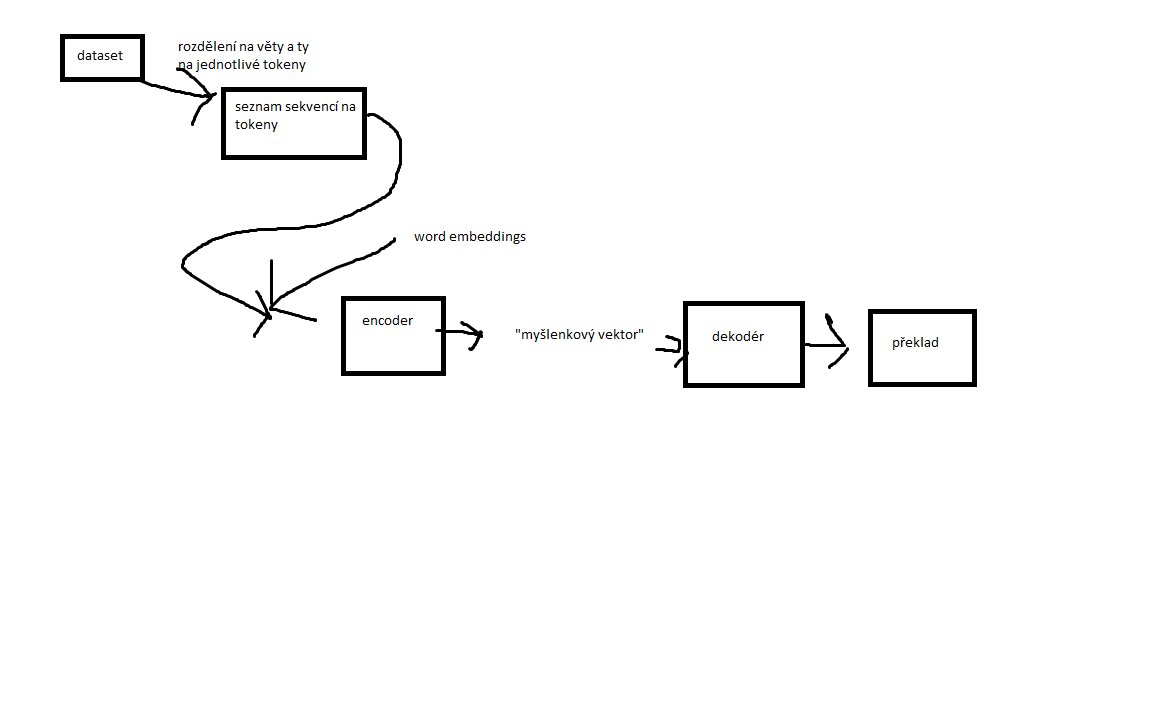
\includegraphics[width=1.0\linewidth]{img/draft.png}}
    \end{center}
	\caption{schéma návrhu systému pro překlad}
	\label{img:draft}
\end{figure}


\chapter{Související teorie a pojmy}
Účelem této kapitoly je blíže vysvětlit a rozebrat jednotlivé pojmy a komponenty potřebné pro vytvoření překladového systému. 



\section{Jazykové modely}\label{section:langmodel}
\todo{citace?}
Zatímco u programovacích jazyků existuje jejich formální definice, přesně popisující jejich syntaxy a význam, u přirozených jazyků to tak není. Přirozený jazyk vznikl náhodným způsobem v průběhu staletí a tisíciletí narozdíl od formálně definovaných jazyků, které byly přímo navrženy. Přestože běžný jazyk se řídí nějakými pravidly, existuje značné množství výjimek a odchylek. I napříč tomu si však lidé navzájem rozumí. Problém však je tyto pravidla převést do formálních pravidel, tak aby jim rozuměl počítač. Řešením pro tento problém mohou být jazykové modely, které nevznikají pomocí definice formálních pravidel, ale učením se z příkladů.

Jazykový model udává pro každou větu $w$ jaká je její pravděpodobnost. Respektive pro sekvenci slov $w = w_1, w_2..., w_m$ získá pravděpodobnost podle \ref{figure:probdistr}.

\begin{align}\label{figure:probdistr}
  p(w) = \prod_{i=1}^{m} p(w_i|w_{<i})
\end{align}

Pro každé slovo $w_i$ ze sekvence určí jaké je jeho podmíněná pravděpodobnost v případě, že se před ním nachází slova $w_i$.

Ve výsledku tak jazykový model umožní zhodnotit přirozenost věty a generovat text podobný tomu, na kterém byl model nacvičen \cite{nmtTutorial}.

\begin{description}
  \item[Zhodnocení přirozenosti] Pomocí jazykového modelu je možné pro větu $w$ zhodnotit, jak moc je přirozená nebo-li jak moc je pravděpodobné, že by takováto věta mohla existovat v textu na kterém byl model nacvičen.
  \item[Generování textu] Protože model umožňuje pro každé slovo $w_i$ získat pravděpodobnost následujícího slova $w_{i+1}$, je takto možné generovat náhodný, přirozeně (vůči zdrojovému textu) vypadající text. Což je přesně potřeba pro generování překladů.
\end{description}


\todo{jazykove modely v kontextu machine translation, generovani jazyku}



Handling Unknown Words \cite{nmtTutorial}

\subsection{N-gram}
\subsection{log-linear}


\subsection{Word embeddings}\label{section:embeddings}
\todo{souvislost s jazykovymy modely}

\todo{více v sekci ... .. a tam budou obrázky, rovnice, vysvětlení...}

\begin{figure}
    \begin{center}
            \tmpframe{
\includegraphics[width=0.5\linewidth]{img/placeholder.pdf}}
    \end{center}
	\caption{One image. \todo{Napsat pořádný titulek}}
	\label{img:TODO}
\end{figure}

Zmíním co existuje za druhy, lehce jejich rozdíly a vznik (co jsou zač) a pak se víc rozepíšu o fasttextu, protože to je ten co jsem použil (rovnice a kdesi cosi)
\begin{itemize}
  \item word2vec
  \item glove
  \item fasttext
\end{itemize}

\section{Rekurentní neuronové sítě}\label{section:rnn}
V této kapitole je popsán základní koncept rekurentních neuronových sítí (RNN\footnote{z anglického recurrent neural network}), jejich srovnání s běžnými neuronovými sítěmi a dále pak popis upravených variant RNN -- LSTM \ref{section:LSTM} a GRU \ref{section:GRU}. Sekce volně vychází z práce \cite{nmtThesis}.\\


RNN (Elman \cite{rnn}) jsou známé již přes dvě desítky let. Úspěšně jsou však používány až v posledních letech a to hlavně díky vyššímu výpočetnímu výkonu a většímu objemu trénovacích dat, který je v současné době dostupný a také, díky většímu výkonu, zpracovatelný. Tento druh neuronových sítí je obzvlášť vhodný například pro rozpoznávání psaného písma, rozpoznávání řeči, v kombinaci s konvolučními neuronovými sítěmi pro generování popisků obrázků a co je nejvíce zajímavé pro tuto práci, pro tvorbu jazykových modelů, generátorů textu a pro překlad.

Jejich hlavních výhodou oproti původním dopředným neuronovým sítím je jejich schopnost držet si vnitřní stav napříč časem. Dopředná neuronová síť pracuje vždy s aktuální hodnotou $x$ na vstupu, pro kterou pomocí vah $W$ získá výstup $y$ (rovnice \ref{figure:basic-nn}).

\begin{align}\label{figure:basic-nn}
  y = f (x, W)
\end{align}

Pokud pak takováto síť pracuje s nějakou sekvencí měnící se v čase, například se slovy v rámci jedné věty, pro každé slovo na vstupu $x_t$, kde $t$ znázorňuje čas (pozici) slova ve větě, použije stejné váhy pro získání výstupu $y_t$ a nezjistí ani nezachová žádnou úvahu o vzájemném vztahu těchto slov.

RNN tento problém řeší zavedením vnitřního stavu $h_t$ a smyčky (obrázek \ref{img:rnn-rolled}). Vstupem dalšího stavu je vždycky výstup ze stavu minulého. Pro každé $x_t$ ze sekvence se tedy nyní může získat výstup $y_t$ pomocí vnitřního stavu $h_t$ z předchozího kroku $t$ (rovnice \ref{figure:rnn}. Přičemž počáteční stav  $h_0$ je obvykle nastaven na nulu.

\begin{align}\label{figure:rnn}
  h_t = f (x_t, h_{t-1})
\end{align}

\begin{figure}[h]
    \begin{center}
            \tmpframe{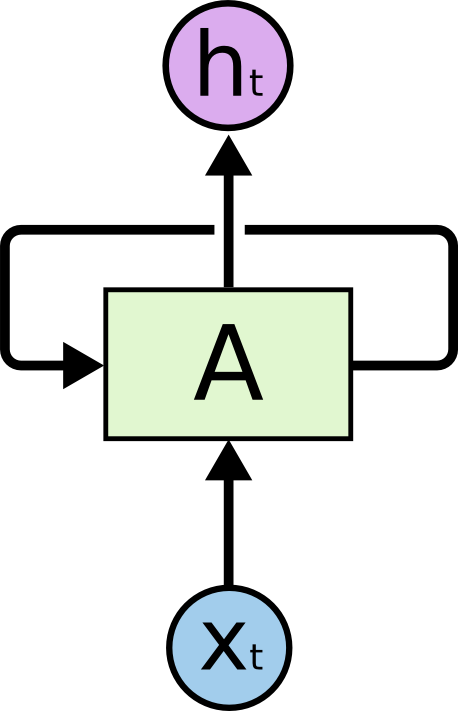
\includegraphics[width=0.3\linewidth]{img/RNN-rolled.png}}
    \end{center}
	\caption{Recurrent Neural Networks have loops. \todo{vlastni obrázek nebo citace \url{http://colah.github.io/posts/2015-08-Understanding-LSTMs/} }}
	\label{img:rnn-rolled}
\end{figure}

Funkce $f$ z rovnice \ref{figure:rnn} je nelineární funkcí a nejčastěji se používá jedna z funkcí \emph{sigmoid}, \emph{tanh} nebo \emph{relu} \ref{img:functions}. \todo{lepe popsat jednotlivé funkce a jejich výhody/nevýhody}

\begin{figure}[h]
    \begin{center}
            \tmpframe{
\includegraphics[width=0.3\linewidth]{img/placeholder.pdf}}
            \tmpframe{
\includegraphics[width=0.3\linewidth]{img/placeholder.pdf}}
            \tmpframe{
\includegraphics[width=0.3\linewidth]{img/placeholder.pdf}}
    \end{center}
	\caption{\todo{vedle sebe obrazky funkci relu, tanh, sigmoid, idealne tri ruzny captions}}
	\label{img:functions}
\end{figure}


\begin{align}\label{figure:softmax}
  \sigma (\mathbf {z} )_{j}={\frac {e^{z_{j}}}{\sum _{k=1}^{K}e^{z_{k}}}}
\end{align}


\begin{figure}[h]
    \begin{center}
            \tmpframe{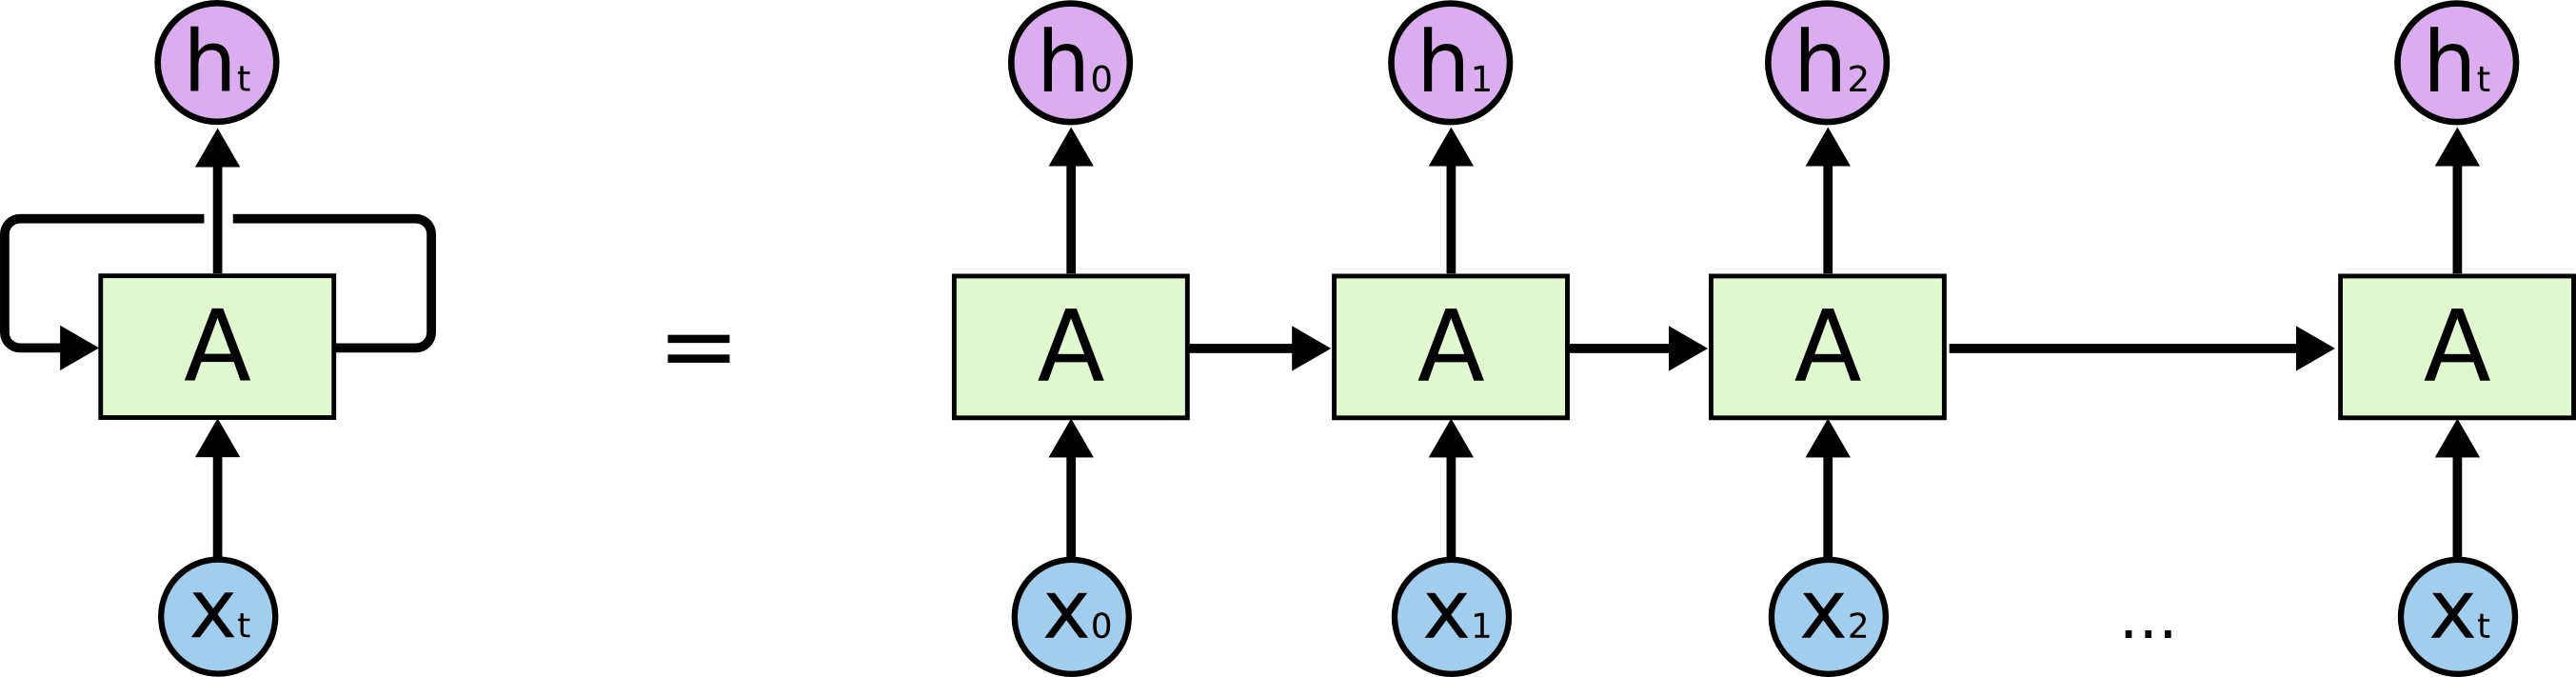
\includegraphics[width=1.0\linewidth]{img/RNN-unrolled.png}}
    \end{center}
	\caption{A recurrent neural network and the unfolding in time of the computation involved in its forward computation. \todo{vlastni obrázek nebo citace \url{http://colah.github.io/posts/2015-08-Understanding-LSTMs/} }}
	\label{img:rnn}
\end{figure}

\todo{doplnit rovnice a vysvětlení jak se to aplikuje dál, stejně tak obrázky s unrolled rnn a popisem toho jak zachovává nějakou informaci (třeba že podstatné jméno je mužské) skrze jednotlivé kroky (i když ne úplně přes vzdálené a tím se dostanu k long term dependencies)}


\todo{trénování rnn, back propagation through time, have difficulties (\url{http://proceedings.mlr.press/v28/pascanu13.pdf}) learning long term dependencies}
\todo{loss computing}
\todo{gradient computing}
\todo{související vanishing a exploding gradient problem popsáno v \cite{gradientProblems}, je to docela popsany i v nmtTutorial}
\todo{predchazeni vanish/exploding - lstm a gru, ktery s tim nejak pocitaji. Regularization - vysvětlit co to je}

\todo{zvlášť neuronky a to jakým způsobem se učí/optimlizují(gradient..) a pak až konkrétně rekurentní nebo rovnou rekurentní?}
\todo{deep, bi-directional}


\subsection{LSTM}\label{section:LSTM}
LSTM (Long short term memory \cite{LSTM} je varianta RNN řešící problém mizejícího gradientu a vzdálených závislostí \todo{lepší překlad pro long term dependencies?}.

\begin{align}
    f_{t}&=\sigma _{g}(W_{f}x_{t}+U_{f}h_{t-1}+b_{f})\\
    i_{t}&=\sigma _{g}(W_{i}x_{t}+U_{i}h_{t-1}+b_{i})\\
    o_{t}&=\sigma _{g}(W_{o}x_{t}+U_{o}h_{t-1}+b_{o})\\
    c_{t}&=f_{t}\circ c_{t-1}+i_{t}\circ \sigma_{c}(W_{c}x_{t}+U_{c}h_{t-1}+b_{c})\\
    h_{t}&=o_{t}\circ \sigma _{h}(c_{t})
\end{align}

\subsection{GRU}\label{section:GRU}


\subsection{Trénování}
\subsection{Global optimization methods viz wiki on RNN}




\section{Modely seq2seq}
\blind{2}
\begin{figure}
    \begin{center}
            \tmpframe{
\includegraphics[width=0.5\linewidth]{img/placeholder.pdf}}
    \end{center}
	\caption{One image. \todo{Napsat pořádný titulek}}
	\label{img:TODO}
\end{figure}
\subsection{Encoder-decoder architektura}
\begin{figure}
    \begin{center}
            \tmpframe{
\includegraphics[width=0.5\linewidth]{img/placeholder.pdf}}
    \end{center}
	\caption{One image. \todo{Napsat pořádný titulek}}
	\label{img:TODO}
\end{figure}
\blind{3}



Ne jako samostatná kapitola, ale v rámci nějaké (asi implementace) bych udělal itemize a nebo přinejmenším aspon zběžně popsal proč jsem zvolili Keras.
\emph{Frameworky}
\begin{itemize}
  \item Tensorflow
  \item Theano
  \item CNTK
  \item Keras
\end{itemize}


\chapter{Implementace}
Naprogramoval jsem.
Posbíral jsem data.
Pustil jsem to.
Výsledky jsou takové.
Je to tak a tak rychlé.

\section{Baseline systém v Moses}
\todo{Jak rozlišit návrh a realizaci?}
\blind{3}

\section{Dataset/y}
Jejich struktura, jak je zpracuji a použiji
\blind{2}
\begin{figure}
    \begin{center}
            \tmpframe{
\includegraphics[width=0.5\linewidth]{img/placeholder.pdf}}
    \end{center}
	\caption{One image. \todo{ukázka ze souborů různých jazyků z jednoho datasetu}}
	\label{img:TODO}
\end{figure}


\subsection{Bucketing}
A padding. Rozdělení sekvencí na skupiny podle délky, abych nepaddingoval zbytečně a tím neplýtval výkon.

\section{popis fungování systému a jednotlivých tříd}

\chapter{Experimenty a vyhodnocení}
\section{skóre BLEU}
\blind{1}
\todo{vysazet hezky vzorce}



\chapter{Závěr}
\begin{itemize}
  \item Autor se ohlíží za tím, co udělal: „V práci je. Hlavní úspěchy jsou. Důležitými výsledky jsou. Podařilo se.“
  \item Autor uvede nápady, které nestihl realizovat v podobě možností pokračování: „Ještě by šlo zkusit. Kdybych byl na začátku věděl, co vím teď, dělal bych.“
  \item Autor (ve vlastním zájmu) rekapituluje, jak bylo naplněno zadání práce.
\end{itemize}

\textbf{Plány do budoucna}
\begin{itemize}
    \item použití bidirectional první vrstvy encoderu, pro lepší zachování contextu \cite{googleBridgingGap} na místo použití obrácených vstupů
    \item použití wordpieces \cite{googleBridgingGap} místo celých slov pro lepší handling rare words
    \item přidat attention \cite{attention}
    \item přidat beam search \cite{nmtTutorial}, sehnat původní článek co přinesl beam search
\end{itemize}
 % viz. obsah.tex / see obsah.tex

  % Pouzita literatura / Bibliography
  % ----------------------------------------------
\ifslovak
  \makeatletter
  \def\@openbib@code{\addcontentsline{toc}{chapter}{Literatúra}}
  \makeatother
  \bibliographystyle{bib-styles/czechiso}
\else
  \ifczech
    \makeatletter
    \def\@openbib@code{\addcontentsline{toc}{chapter}{Literatura}}
    \makeatother
    \bibliographystyle{bib-styles/czechiso}
  \else
    \makeatletter
    \def\@openbib@code{\addcontentsline{toc}{chapter}{Bibliography}}
    \makeatother
    \bibliographystyle{bib-styles/englishiso}
  %  \bibliographystyle{alpha}
  \fi
\fi
  \begin{flushleft}
  \bibliography{xholcn01-dp-20-literatura-bibliography}
  \end{flushleft}

  % vynechani stranky v oboustrannem rezimu
  % Skip the page in the two-sided mode
  \iftwoside
    \cleardoublepage
  \fi

  % Prilohy / Appendices
  % ---------------------------------------------
  \appendix
\ifczech
  \renewcommand{\appendixpagename}{Přílohy}
  \renewcommand{\appendixtocname}{Přílohy}
  \renewcommand{\appendixname}{Příloha}
\fi
\ifslovak
  \renewcommand{\appendixpagename}{Prílohy}
  \renewcommand{\appendixtocname}{Prílohy}
  \renewcommand{\appendixname}{Príloha}
\fi
%  \appendixpage

% vynechani stranky v oboustrannem rezimu
% Skip the page in the two-sided mode
%\iftwoside
%  \cleardoublepage
%\fi

\ifslovak
%  \section*{Zoznam príloh}
%  \addcontentsline{toc}{section}{Zoznam príloh}
\else
  \ifczech
%    \section*{Seznam příloh}
%    \addcontentsline{toc}{section}{Seznam příloh}
  \else
%    \section*{List of Appendices}
%    \addcontentsline{toc}{section}{List of Appendices}
  \fi
\fi
  \startcontents[chapters]
  \setlength{\parskip}{0pt}
  % seznam příloh / list of appendices
  % \printcontents[chapters]{l}{0}{\setcounter{tocdepth}{2}}

  \ifODSAZ
    \setlength{\parskip}{0.5\bigskipamount}
  \else
    \setlength{\parskip}{0pt}
  \fi

  % vynechani stranky v oboustrannem rezimu
  \iftwoside
    \cleardoublepage
  \fi
  % Tento soubor nahraďte vlastním souborem s přílohami (nadpisy níže jsou pouze pro příklad)
% This file should be replaced with your file with an appendices (headings below are examples only)

% Umístění obsahu paměťového média do příloh je vhodné konzultovat s vedoucím
% Placing of table of contents of the memory media here should be consulted with a supervisor
%\chapter{Obsah přiloženého paměťového média}

%\chapter{Manuál}

%\chapter{Konfigurační soubor} % Configuration file

%\chapter{RelaxNG Schéma konfiguračního souboru} % Scheme of RelaxNG configuration file

%\chapter{Plakát} % poster

\chapter{Poznámky} \label{kapitola:poznamky}

\section{TODOs}
http://www.statmt.org/moses/?n=Moses.Releases \ref{moses}

data bych doporucil open subtitles http://opus.lingfil.uu.se/

subtitles projet aligmentem.. oscorovat pary vet a pak vyfiltrovat malo pravdepodobne -> rozumna data\\
stahnuto, zkusil jsem projet moses => po 24 hodinach zaplnilo cely disk a nebylo hotovo. Filtrovani pomoci  -score-options="-MinScore?

wmt vysledky http://www.statmt.org/wmt17/results.html ? BLEU


\section{Pseudo zadani}

chapu to tak, ze: nejdriv projedu kazde slovo na vstupu skrz prepripraveny nauceny veci od facebooku do embeddings a to pak teprve posilam do encoderu. Ten mi z toho pak vyhodi context (thought) vector\\
pouziju bidirectional LSTM (RNN) + attention + beam search\\
kazdej vstup (veta) je zarovnana (padding) na nejakou delku (bud se to doplni nebo naopak oreze), potom se z toho udela embeddings s pouzitim pretrained, potom se prozene encoderem, ziskam context, ten se prozedene dekoderem (s pomoci attention)\\
src input bude reversed sequence, protoze to podle nekterych clanku funguje lip, nevim jestli nestaci pouzit bi-directional LSTM\\

podle thesis je mozny pouzit hybridni model, generovat znama slova po slovech (ne po jednotlivych characterech) a neznama slova po jednotlivych znacich (takze vystupem muze byt o slovo mimo slovnik ze kteryho se sit ucila)\\

myslel jsem ze vystupem je embeding, ze kteryho se napr. podle vzdalenosti zjisti vysledne slovo, ale mozna je spis vystupem one hot encoding velikosti output slovniku a embeddings se pouzivaji jenom v prubeznych vrstvach

\section{Kapitoly}
\begin{itemize}
  \item what is machine learning
  \item machine learning druhy (odvozovani ze znalosti, feature/representation, deep learning)
  \item popis ruznych neuronovych siti - CNN (images), structural?/standard NN (?), RNN(audio/translation), LSTM (translation)?,
  \item hyperparameters
  \item popis ruznych zpusobu strojoveho prekladu textu
  \item popis frameworku? na neuronky
  \item Tensors
  \item activation functions
  \item Tools - moses
  \item frameworks - google tensorflow, microsoft CNTK, theano, keras (with usage of tensorflow/cntk/theano), tf.contrib.Keras + tf
  \item pretrained embeddings - facebook, word2vec, glove
\end{itemize}


\section{Facebook pretrained word vectors}
obsahuji textovou verzi - slovo a jeho vector a binarni verzi ve formatu fastText
\url{https://github.com/facebookresearch/fastText/blob/master/pretrained-vectors.md}\\
\url{https://blog.manash.me/how-to-use-pre-trained-word-vectors-from-facebooks-fasttext-a71e6d55f27}\\
\url{https://www.quora.com/What-is-the-main-difference-between-word2vec-and-fastText}

\section{Moses}
\begin{itemize} \label{moses}
  \item UKAZKA JAK TO POUZIVA GOOGLE TUTORIAL \url{https://github.com/tensorflow/nmt/blob/master/nmt/scripts/wmt16_en_de.sh}
  \item statistical machine translation (SMT) or probably syntax based translation or factored translation
  \item data preparation
  \begin{itemize}
    \item tokenisation: This means that spaces have to be inserted between (e.g.) words and punctuation.
    \item truecasing: The initial words in each sentence are converted to their most probable casing. This helps reduce data sparsity.
    \item cleaning: Long sentences and empty sentences are removed as they can cause problems with the training pipeline, and obviously mis-aligned sentences are removed.
  \end{itemize}
  \item co zatim zkousim, rucne postupne jednotlive kroky
  \begin{itemize}
    \item mam data z http://opus.lingfil.uu.se/ pro cs (Czech)/en (English) pro moses, tzn tri soubory moses.cs-en.cs, moses.cs-en.en, moses.cs-en.ids
    \item tokenizace
    \begin{lstlisting}
    ~/mosesdecoder/scripts/tokenizer/tokenizer.perl -l en \
    < /media/sf_DPbigFiles/OpenSubtitles2016-moses.cs-en.en \
    > /media/sf_DPbigFiles/OpenSubtitles2016-moses.cs-en.tokenized.en
    \end{lstlisting}
    \item nauceni truecaser modelu
    \begin{lstlisting}
    ~/mosesdecoder/scripts/recaser/train-truecaser.perl \
    --model /media/sf_DPbigFiles/truecase-model.en \
    --corpus /media/sf_DPbigFiles/OpenSubtitles2016-moses.cs-en.tokenized.en
    \end{lstlisting}
    \item truecased
    \begin{lstlisting}
    ~/mosesdecoder/scripts/recaser/truecase.perl \
    --model /media/sf_DPbigFiles/truecase-model.en \
    < /media/sf_DPbigFiles/OpenSubtitles2016-moses.cs-en.tokenized.en \
    > /media/sf_DPbigFiles/OpenSubtitles2016-moses.cs-en.tokenized.truecased.en
    \end{lstlisting}
    \item cleaning
    \begin{lstlisting}
    ~/mosesdecoder/scripts/training/clean-corpus-n.perl /media/sf_DPbigFiles/OpenSubtitles2016-moses.cs-en.tokenized.truecased cs en /media/sf_DPbigFiles/OpenSubtitles2016-moses.cs-en.tokenized.truecased.cleaned 1 80
    \end{lstlisting}
    \item language model training
    \begin{lstlisting}
    /media/sf_DPbigFiles/languagemodel$ ~/mosesdecoder/bin/lmplz -o 3 < /media/sf_DPbigFiles/OpenSubtitles2016-moses.cs-en.tokenized.truecased.cleaned.en > OpenSubtitles2016-moses.cs-en.arpa.en
    \end{lstlisting}
    \item binarizing for faster loading
    \begin{lstlisting}
    ~/mosesdecoder/bin/build_binary OpenSubtitles2016-moses.cs-en.arpa.en OpenSubtitles2016-moses.cs-en.binary.en
    \end{lstlisting}
    \item training - ZKUSIT PUSTIT BEZ PARAMETRU rika to pak ty jednotlivy stepy co chci udelat
    \begin{lstlisting}
    ~/mosesdecoder/scripts/training/train-model.perl -root-dir . --corpus /media/sf_DPbigFiles/OpenSubtitles2016-moses.cs-en.tokenized.truecased.cleaned --f cs --e en -external-bin-dir ~/mosesdecoder/tools/ -cores 4 -parallel -lm 0:3:/media/sf_DPbigFiles/languagemodel/OpenSubtitles2016-moses.cs-en.binary.en
    \end{lstlisting}
    \begin{lstlisting}
    with mgiza++
    ~/mosesdecoder/scripts/training/train-model.perl -root-dir train -corpus ~/corpus/news-commentary-v8.fr-en.clean -f fr -e en -alignment grow-diag-final-
    and -reordering msd-bidirectional-fe -lm 0:3:$HOME/lm/news-commentary-v8.fr-en.blm.en:8 -external-bin-dir ~/mosesdecoder/tools -cores 4 -parallel -mgiza -mgiza-cpus 4
    \end{lstlisting}
  \end{itemize}
  OpenSubtitles2016-moses.cs-en.cs/en jsou moc velky, zkusim vzit mensi cast (prvnich x radku) a natrenovat to s tim. Puvodni velka obsahuje 33896950 radku.

  \begin{itemize}
    \item pouziti EMS - Experiment Management System, ktery obdrzi konfiguracni soubor a resi si jednotlive kroky a skripty sam
    \item nainstaloval jsem xming, potreba pred spustenim skriptu "export DISPLAY=:0"
    \item ~/mosesdecoder/scripts/ems/experiment.perl -config config.toy -exec
    \item spadlo to na step EVALUATION:test:nist-bleu crashed step EVALUATION:test:nist-bleu-c crashed
    \item takze asi zustanu u rucne postupnych prikazu - vytvoren vlastni skrupt runAll.sh. bash -x ./runAll.sh \url{http://www.statmt.org/moses/?n=Moses.Baseline}
  \end{itemize}
\end{itemize}

\section{odkazy}
\url{https://en.wikipedia.org/wiki/Language_model}

\begin{itemize}
    \item RBMT \url{https://en.wikipedia.org/wiki/Rule-based_machine_translation}
    \item SMT \url{https://en.wikipedia.org/wiki/Statistical_machine_translation}
    \item nejaky dalsi...?
    \item neuronka (GNMT, Transfomer)
\end{itemize}

computing BLEU score in python using ntlk lib \url{http://www.nltk.org/_modules/nltk/align/bleu.html}

research at google - machine translation articles \\ \url{https://research.google.com/pubs/MachineTranslation.html}\\
\url{https://en.wikipedia.org/wiki/Google_Neural_Machine_Translation}\\

\url{https://research.googleblog.com/2016/09/a-neural-network-for-machine.html}\\

\url{https://research.googleblog.com/2017/06/accelerating-deep-learning-research.html} \\
\url{https://research.googleblog.com/2017/07/building-your-own-neural-machine.html} \\
\url{https://research.googleblog.com/2017/04/introducing-tf-seq2seq-open-source.html}\\

\textbf{BUCKETING AND PADDING IN TENSOR FLOW}
\url{https://www.tensorflow.org/tutorials/seq2seq#bucketing_and_padding}

\textbf{neural machine translation tutorial acl 2016}
\url{https://sites.google.com/site/acl16nmt/home}

\textbf{chat bot in keras}
\url{https://github.com/saurabhmathur96/Neural-Chatbot}

\url{https://en.wikipedia.org/wiki/Language_model}

\section{knihovny nad tensorflow}
\begin{itemize}
  \item \url{google.github.io/seq2seq} - A general-purpose encoder-decoder framework for Tensorflow, pomoci konfiguraci, snadne vytvoreni komplexnich seq2seq modelu, pouzity pro clanek Massive Exploration of Neural Machine Translation Architectures. NENI UDRZOVANO z https://gitter.im/tensor2tensor/Lobby -  google/seq2seq is not maintained. If you're just starting, read this first https://github.com/tensorflow/nmt and read papers, the one for this repo too.
  \item \url{github.com/tensorflow/tensor2tensor}- A library for generalized sequence to sequence models, pomoci konfiguraci (vyber ruznych modulu a moznost vytvoreni vlastni), asi relativne snadny vytvoreni ruznych (obecnych, nejen seq2seq) modelu. VYPADA TO ROZUMNE
  \item \url{github.com/tensorflow/nmt} - zatimco T2T uz je hlavne skladacka predpripravenych veci, tenhle tutorial ukazuje jak vyrobit v tensorflow od pocatku vlastni model
\end{itemize}


\section {Neural Machine Translation (seq2seq) Tutorial}
\url{https://github.com/tensorflow/nmt} podle \url{https://github.com/lmthang/thesis}, uzitecnej clanek

\begin{itemize}
  \item nmt model can differ in terms of \emph{directionality} uni/bi, \emph{depth} single/multi layer, \emph{type} vanilla RNN/LSTM/GRU
  \item In this tutorial, we consider as examples a deep multi-layer RNN which is unidirectional and uses LSTM as a recurrent unit.
  \item time-major format znamena ze prvni parameter je max\_encoder\_time a druhy batchsize, u batch-major je to naopak
  \item DECODER teda funguje tak, ze dostava 1. vysledek z encoderu, tim vi z ceho preklada a k tomu 2. nejdriv znak <s> pro zacatek dekodovani a v dalsich casovych stepech pak pri treningu ty spravne slova prekladu a pri pouziti pak ty slova co sam vygeneruje. Je to dobre popsany v \url{https://github.com/tensorflow/nmt#inference--how-to-generate-translations}
  \item ukazka z tutorialu v gitbashi spadne s encoding problemem, v cmd ne
  \item ukazka spadne na nedostatku pameti, je potreba zmenit parametry. (po kazde zmene radsi smazat slozku nmt\_model).
      \begin{lstlisting}
pro cmd
python -m nmt.nmt ^
    --src=vi --tgt=en ^
    --vocab_prefix=nmt_data/vocab  ^
    --train_prefix=nmt_data/train ^
    --dev_prefix=nmt_data/tst2012  ^
    --test_prefix=nmt_data/tst2013 ^
    --out_dir=nmt_model ^
    --num_train_steps=1000 ^
    --steps_per_stats=100 ^
    --num_layers=2 ^
    --num_units=32 ^
    --batch_size=64 ^
    --dropout=0.2 ^
    --metrics=bleu
    \end{lstlisting}
vyzkousim jak to funguje
\begin{lstlisting}
python -m nmt.nmt ^
    --out_dir=nmt_model ^
    --inference_input_file=nmt_data/my_infer_file.vi ^
    --inference_output_file=nmt_model/output_infer
\end{lstlisting}
\end{itemize}

\section{old tensorflow seq2seq tutorial}
\url{https://www.tensorflow.org/tutorials/seq2seq}
\begin{lstlisting}
old seq2seq tutorial G:\Dropbox\vecicky\python\tensorFlow\RNNtutorial\translate
python translate.py ^
  --data_dir=nmt_data --train_dir=train ^
  --from_vocab_size=100 --to_vocab_size=100 ^
  --from_train_data=nmt_data/OpenSubtitles2016-moses-10000.cs-en-tokenized.truecased.cleaned.cs ^
  --to_train_data=nmt_data/OpenSubtitles2016-moses-10000.cs-en-tokenized.truecased.cleaned.en ^
  --size=256 --batch_size=32 --num_layers=1

spadlo to zas na pameti, zkusim mensi size a tak

https://github.com/tensorflow/tensorflow/issues/11157
I suffered exactly the same problem.
I just passed the error by modifying 2 lines of the following seq2seq.py file from Tensorflow.

file: Anaconda3\Lib\site-packages\tensorflow\contrib\legacy_seq2seq\python\ops\seq2seq.py
848 #encoder_cell = copy.deepcopy(cell)
849 encoder_cell = core_rnn_cell.EmbeddingWrapper(
850 cell, #encoder_cell,

preklad
python translate.py --decode --data_dir=nmt_data --train_dir=train ^
    --from_vocab_size=100 --to_vocab_size=100
\end{lstlisting}

\section{Tensor2Tensor}
\url{github.com/tensorflow/tensor2tensor}
\begin{itemize}
  \item po instalaci na windows nefunguji pripravene bin programy podle tutorialu (jako t2t-trainer). Je potreba stahnout si je z repositare a poustet rucne - python t2t-trainer
  \begin{lstlisting}
python bin/t2t-trainer.py ^
  --generate_data ^
  --data_dir=walktrough/t2t_data ^
  --problems=translate_enmk_setimes32k ^
  --model=transformer ^
  --hparams_set=transformer_base_single_gpu ^
  --output_dir=walktrough/t2t_train/base ^
  --hparams="batch_size=64"

  a stejne to spadne s
  InternalError (see above for traceback): Blas SGEMM launch failed : m=90, n=1536, k=512\\
  zmenil jsem flags.DEFINE_float("worker_gpu_memory_fraction", 0.35,
                   "Fraction of GPU memory to allocate.") v souboru knihovny tensor2tensor trainer_utils.py z 0.95 na 0.35 a stejne to spadne na OOM
  \end{lstlisting}
\end{itemize}

\section{transformer, tensorFlow}
\begin{itemize}
    \item googls novel neural architecture - Transformer better than GNMT (google neural machine translation) \url{https://research.googleblog.com/2017/08/transformer-novel-neural-network.html}
    \item tensor2tensor \url{https://github.com/tensorflow/tensor2tensor/}
    \item t2t \url{https://research.googleblog.com/2017/06/accelerating-deep-learning-research.html}
    \item Train set for training, validation set for hyperparameters tuning, test set for testing how good
\end{itemize}

transformer - uses only attention and gets rid of recurrence and convolution. What exactly is and does recurrence and convolution (in context of neural networks)? Probably another thing that could be written in the theoretical part.



\section{vypisky z deep learning book}
\begin{itemize}
    \item uvod a historie, jak se postupne menily a jaky byly ruzny druhy machine learning
    \item machine learning basics
    \begin{itemize}
      \item klasifikace
      \item klasifikace s chybejicimi vstupy
      \item regrese
      \item transription
      \item MACHINE TRANSLATION
      \item structured output
      \item anomaly detection
      \item Synthesis and sampling
      \item Imputation of missing values
      \item Denoising
      \item Density estimationorprobability mass function estimation
    \end{itemize}
    \item Task, Performance measure, Expericen..to co to ma delat, cim a jak se zmeri jak dobre to dela, cinnost na ktere se to nauci
    \item unsupervised - nema popisky a pocitac se snazi sam z dat urcit nejake zavery - treba clustering, supervised - ty maji label pro data v data setu, takze se nauci pro ktere x je jake y a pak se snazi odvodit y pro dalsi nahodne x, ktere se jim predhodi
    \item underfitting, overfitting
    \item train error (chybovost na trainovacim data setu) vs generalization error (chybovost na testovacim datasetu)
    \item regularization
    \item hyperparameters
    \item train vs test vs validation set
    \item regression - ziskavame nejakou hodnotu na zaklade parametru, klasifikace - rozrazujeme do presne danych trid
\end{itemize}

5.4 Estimators, Bias and Variance

\section{coursera deeplearning}
vypisky z \url{https://www.coursera.org/learn/neural-networks-deep-learning}
\begin{itemize}
  \item RELU - rectified linear unit, nahrazuje sigmoid funkci, protoze se nad ni rychleji uci
  \item structured data - tabulky informaci, kazdej sloupec je jedna feature (age, bedooorms, price) X unstructured data - obrazky, hudba, text
  \item logistic regression - jaka je procentualni sance ze x na vstupu = nejake vystupni y (asi jenom jedno konkretni), je to binarni klasifikace. Na rozrazeni do 0-1 pouziva sigmoid funkci
  \item cost function pro logistickou regresi - prumer loss funkce nad celym trenovacim setem
  \item vektor v matici je jako jeden sloupec
  \item (VEKTORIZACE) nasobeni vektoru v maticich misto ve smycce je radove rychlejsi! (numpy.dot), SIMD instrukce (single instruction, multiple data)
  \item broadcasting (v pythonu) vstupni hodnotu (at uz matici nebo skalar) namnozi takovym zpusobem, aby sla pouzit v operaci s matici
  \item The main steps for building a Neural Network are:
  \begin{itemize}
    \item Define the model structure (such as number of input features)
    \item Initialize the model's parameters
    \item Loop:
    \item Calculate current loss (forward propagation)
    \item Calculate current gradient (backward propagation)
    \item Update parameters (gradient descent)
  \end{itemize}
  \item $Z_{n}^{[l](v)}$ l - index of layer (hidden), v - index of training vector, n - index of node in the layer
  \item activation functions (sigmoid 0-1 better for output layer for binary classification, tanh -1 - 1 better for hidden layers, (leaky) RELU 0/1 even better)
  \item bias can be initialized to zero but weights must be initialized randomly because all the nodes inside layer would have the same weights and would be calculating the same numbers (they would be identical)
\end{itemize}

\section{bridging the gap}
vypisky z Google’s Neural Machine Translation System: Bridging the Gap
between Human and Machine Translation
\begin{itemize}
  \item encoder (LSTM RNN) - transforms a source sentence into a list of vectors, one vector per input symbol; 8 layers
  \item decoder (LSTM RNN) - produces on symbol at a time from the vectors; 8 layers
  \item those two are connected through an attention module - feed forward network with one hidden layer
  \item attention - koukne se pro kazde slovo na jeho okoli a pri prekladu se rozhodne, ktera slovo s tim danym slovem nejvice souvisi a podle toho vybere spravny preklad
  \item residual connections enable to train much deeper networks
  \item neural network model weights can be quantizied to speed up some inference
  \item BLEU score metric
  \item pouziti wordpieces (vylepsuje handlig rare slov), coz umoznuje generovani novych slov jako pri pouziti modelu po jednotlivych pismenech, ale je to efektivnejsi jako pri pouziti celych slov
  \item Using wordpieces gives a good balance between the flexibility of single characters and the efficiency of full words for decoding, and also sidesteps the need for special treatment of unknown words.
\end{itemize}

\section{deep learning thesis}
vypisky z thesis(nmtTutorialBasedOnThis) https://github.com/lmthang/thesis
\begin{itemize}
  \item Language modeling is an important concept in natural language processing to allow one to do word prediction, i.e., guessing which word will come next given a preceding context.
  \item it does so by predicting next words in a text given a history of previous words.
  \item word embeddings are used instead of one-hot representation for words (long vector, one value for each word in vocabulary, 0 meaning false and 1 meaning true). Word embeddings has the same meaning value but are much smaller matrices.
\end{itemize}

\section{clanek sequence to sequence learning with nn}
\begin{itemize}
  \item normal deep neural network models are excellent on many task, but not on mapping sequence to sequence.
  \item use LSTM to map input sequence to thought vector (encoder) then decoder to map to target sequence
  \item reversing order of words in all source sentences improves LSTM's performance markedly because of many short term dependencies
  \item Despite their flexibility and power, DNNs can only be applied to problems whose inputs and targets can be sensibly encoded with vectors of fixed dimensionality.
  \item The goal of the LSTM is to estimate the conditional probability
  \item again USES DATASET English to French translation task from the WMT 14 dataset

\end{itemize}

\section{clanek unsupervised machine translation using monolingual corpora only}
\begin{itemize}
  \item model that takes sentences from monolingual corpora in two different languages and maps them into the same latent space
  \item By learning to reconstruct in both languages from this shared feature space, the model effectively learns to translate without using any labeled data.
  \item TWO WIDELY USED DATASETS and two language pairs - zkusit zjistit ktery jsou widely used datasets a pouzit je taky
  \item the model has to be able to reconstruct a sentence in a given language from a noisy version of it, as in standard denoising auto-encoders
  \item The model also learns to reconstruct any source sentence given a noisy translation of the same sentence in the target domain, and vice versa.
  \item jak vyuziva decoder word embeddings corresponddujici k danemu jazyku?
  \item The encoder is a bidirectional-LSTM which returns a sequence of hidden states z. At each step, the decoder, which is an LSTM, takes the previous hidden state, the current word and a context vector given by a weighted sum over the encoder states.
  \item jak funguje naivni inicializace s unsporvised vytvorenym word by word prekladem?
  \item chapu to tak, ze preklad funguje nasledovne - vezme se source veta v source jazyce, prelozi se translation modelem M (ktery je, nevim co?) a vznikne tak ne uplne povedeny preklad. Protoze se to predtim ucilo autoencodovat z do stejneho jazyka na poskozenych vetach, tak je nasledovne mozne tento poskozeny preklad prohnat autoencoderem a tim dostat spravny preklad (protoze se to predtim ucilo z pozkozenych vet tvorit spravne vety).
  \item M je nazacatku unsupervised word-by-word translation model using the inferred dictionary
  \item pouzivaji WMT 14 English-French a WMT 16 English-German
  \item \url{http://www.statmt.org/wmt14/translation-task.html}
\end{itemize}

\section{clanek Learning Phrase Representations using RNN Encoder–Decoder for Statistical Machine Translation}
\begin{itemize}
  \item The encoder maps a variable-length source sequence to a fixed-length vector, and the decoder maps the vector representation back to a variable-length target sequence.
  \item The two networks are trained jointly to maximize the conditional probability of the target sequence given a source sequence.
  \item RNN Encoder–Decoder learns a continuous space representation of a phrase that preserves both the semantic and syntactic structure of the phrase.
  \item RNN is neural network with hidden state h and optional output y which takes variable length input x. $h_t = f(h_{t-1}, x_t)$
  \item After reading the end of the sequence (marked by an end-of-sequence symbol), the hidden state of the RNN is a summary c of the whole input sequence.
  \item baseline model - popsany co jak vybraly za data, WMT14 english-french, SMT system v moses s default settings
\end{itemize}

\url{http://colah.github.io/posts/2015-08-Understanding-LSTMs/}
\section{understanding LSTM networks and }\label{LSTM}
\begin{itemize}
  \item potrebuju pochopit co je vystup encoderu/LSTM, rozdil mezi hidden state a cell(memory) state a co presne vechno se pak z toho pouzije v decoderu viz clanek predtim
  \item url{https://www.quora.com/What-is-the-difference-between-states-and-outputs-in-LSTM}
  \item zakladni RNN si neumi pamatovat veci pres delsi casovej usek (single tanh layer)
  \item LSTM je se reseni - STMs are explicitly designed to avoid the long-term dependency problem
  \item CELL STATE
  \begin{itemize}
    \item The cell state is kind of like a conveyor belt. It runs straight down the entire chain, with only some minor linear interactions. It’s very easy for information to just flow along it unchanged.
    \item The LSTM does have the ability to remove or add information to the cell state, carefully regulated by structures called gates.
    \item Gates are a way to optionally let information through. They are composed out of a sigmoid neural net layer and a pointwise multiplication operation.
    \item The sigmoid layer outputs numbers between zero and one, describing how much of each component should be let through. A value of zero means “let nothing through,” while a value of one means “let everything through!” An LSTM has three of these gates, to protect and control the cell state.
    \item FIRST forget values based on $W_f$, then get learn new values based on $W_i and W_C$ and finally get new cell state from it
  \end{itemize}
  \item OUTPUT $h_t$ is based on cell state and filtered and shifted to -1 and 1 values using another weight $W_o$
  \item pochopil jsem cell state jako stav, ke kteremu se dojde patrne jednim pruchodem/prubehem/iteraci zkrz LSTM vrstvu (takze treba kdyz do toho poslu jednu sequenci), ve kterem se/jaky bunka ma na konci. tzn dostalo to nakou vetu a postupne si to z ni neco bralo a zapominalo a na konci to ma ve svym cell state
  \item zatimco hidden state je output (ktery v pripade encoderu nevim co je)
  \item kde jsou v LSTM vahy ktery se uci? patrne uvnitr tech jednotlivych gate a urcuji prave co si to prenasi mezi krokama sekvence INPUT/OUTPUT/FORGET gate. vaha pro forget layer, pro input gate layer a candidate values
  \item OUTPUT is The vector of outputs from all memory units is the output of the LSTM network.

\end{itemize}

\section{The Unreasonable Effectiveness of Recurrent Neural Networks}
\url{http://karpathy.github.io/2015/05/21/rnn-effectiveness/}
\begin{itemize}
  \item If training vanilla neural nets is optimization over functions, training recurrent nets is optimization over programs.
  \item it is known that RNNs are Turing-Complete in the sense that they can to simulate arbitrary programs (with proper weights).
  \item vanilla RNN (nebo rekneme spis obecne RNN), jeden krok je pronasobeni vah W s vnitrnim hidden stavem h, ten se updatuje kazdy krok pomoci nejake funkce (tanh, v lstm je tam zapominaci a ucici se gate..) a vystupem teda je nasobek W*h
  \item character-level language model: That is, we’ll give the RNN a huge chunk of text and ask it to model the probability distribution of the next character in the sequence given a sequence of previous characters. This will then allow us to generate new text one character at a time.
  \item docela hezky popsana backpropagace v rnn u obrazku s prikladem "hello"
  \item
\end{itemize}

\section{Language models}
\url{https://machinelearningmastery.com/statistical-language-modeling-and-neural-language-models/}
\begin{itemize}
  \item Language modeling is the task of assigning a probability to sentences in a language. […] Besides assigning a probability to each sequence of words, the language models also assigns a probability for the likelihood of a given word (or a sequence of words) to follow a sequence of words (Page 105 Neural Network Methods in Natural Language Processing, 2017.)
  \item Language modeling is the art of determining the probability of a sequence of words. This is useful in a large variety of areas including speech recognition, optical character recognition, handwriting recognition, machine translation, and spelling correction
  \item The use of neural networks in language modeling is often called Neural Language Modeling, or NLM for short.
  \item Neural Language Models (NLM) address the n-gram data sparsity issue through parameterization of words as vectors (word embeddings) and using them as inputs to a neural network. The parameters are learned as part of the training process. Word embeddings obtained through NLMs exhibit the property whereby semantically close words are likewise close in the induced vector space.
  \item The neural network approach to language modeling can be described using the three following model properties, taken from “A Neural Probabilistic Language Model“, 2003.
      Associate each word in the vocabulary with a distributed word feature vector. Express the joint probability function of word sequences in terms of the feature vectors of these words in the sequence. Learn simultaneously the word feature vector and the parameters of the probability function.
\end{itemize}

\section{clanek Neural Machine Translation and Sequence-to-sequence Models:A Tutorial}
\begin{itemize}
  \item n gram models - The parameters of n gram models consist of probabilities of the next word given n 1 previous words
  \item has definition of training/development/test data (3.3)
  \item definition of perplexity
  \item ngram vs log-linear models - log linear models calculate the same probabilty of word given a context, but use feature vector. Feature function takes a context as input and gives feature vector as output - for example identity of a word is a vector that is why all words has unique id. One hot vectors are used
  \item dobrej popis LSTM a celkove RNN
  \item residual connections aby se vyhlo vanishing gradientu
  \item popis batchingu a vyhod ruznych velikosti
  \item muzu v kerasu posilat ruzny delky nebo musim mit vsechny stejne dlouhy s paddingem? to je prece plytvani! mohl bych je rozdelit na ruzny velikosti a volat fit takhle s ruznyma, abych to optimalizoval DNESKA- BUCKETING v tensorflow
  \item dobrej popis encoder-decoder, pouzil bych vzdycky odkaz na puvodni zdroj a podle tohodle pak psal, protoze je to hezky pochopitelny
  \item pouziti beam search misto argmax, ruzny encodovani a ensembling?
  \item vyzkouset nebo popsat proc reverse vstupu nebo zkusit misto toho BI-DIRECTIONAL encoder
  \item takze uz mam do budoucna bidirectional encoder, beam search, bucketing, rare (unknown/oov words)
  \item popsat ruzny optimizery adam/gradient..
\end{itemize}

\section{TENSORFLOW}
\begin{itemize}
  \item NVIDIA GTX 760, CUDA support + cudnn
  \item tensorboard
  \item it is often needed to reduce batch size/unit count, because otherwise there is an resourceExhausted error (memory on GPU is too low?)
\end{itemize}

\section{keras}
\url{https://blog.keras.io/a-ten-minute-introduction-to-sequence-to-sequence-learning-in-keras.html}
detailni rozbor keras blogu
\url{https://machinelearningmastery.com/define-encoder-decoder-sequence-sequence-model-neural-machine-translation-keras/}
\begin{itemize}
  \item pouziva preklad po znacich misto po slovech
  \item LSTM in keras and time distributed layer \url{https://machinelearningmastery.com/timedistributed-layer-for-long-short-term-memory-networks-in-python/}
  \item inference mode as opposed to learning mode where we insert into decoder start tag and the whole correct translation:
    1) Encode the input sequence into state vectors.
    2) Start with a target sequence of size 1 (just the start-of-sequence character).
    3) Feed the state vectors and 1-char target sequence to the decoder to produce predictions for the next character.
    4) Sample the next character using these predictions (we simply use argmax).
    5) Append the sampled character to the target sequence
    6) Repeat until we generate the end-of-sequence character or we hit the character limit.
    \item A Dense output layer is used to predict each character. This Dense is used to produce each character in the output sequence in a one-shot manner, rather than recursively, at least during training. This is because the entire target sequence required for input to the model is known during training. The Dense does not need to be wrapped in a TimeDistributed layer.
    \item we can plot the model to file using keras plot-model, graphviz must be installed (both through pip in python and in windows as binary)
    \item pro musi byt padding a fixed length? \url{https://danijar.com/variable-sequence-lengths-in-tensorflow/}, ale jak teda muze google prekladat libovolne dlouhy vety? rozdeli je na mensi?
    \item c - cell state, h - hidden state, vysvetleno lip v section \ref{LSTM} \url{https://machinelearningmastery.com/return-sequences-and-return-states-for-lstms-in-keras/}
    \item \url{https://stackoverflow.com/questions/44515336/how-do-i-show-both-training-loss-and-validation-loss-on-the-same-graph-in-tensor}
    \item \textbf{WARNING: }in python set(chars) doesn't return the same set everytime, order isnt given in set!! must sort as a list, otherwise on python close, the loaded model weights wouldn't correspond correctly to it!!!!
    \item LSTM stateful \url{https://stackoverflow.com/a/46331227}, zaver - defaultni stateful false je v pohode a kazda sequence ma vlastni novej C state
    \item automatic early stopping based on val\_loss \url{https://stackoverflow.com/questions/43906048/keras-early-stopping}
\end{itemize}

\textbf{embeddings in keras}
\url{https://machinelearningmastery.com/use-word-embedding-layers-deep-learning-keras/}
\begin{itemize}
  \item A word embedding is a class of approaches for representing words and documents using a dense vector representation.
  \item The position of a word within the vector space is learned from text and is based on the words that surround the word when it is used.
  \item The position of a word in the learned vector space is referred to as its embedding.
  \item The keras embedding layer requires that the input data be integer encoded, so that each word is represented by a unique integer. This data preparation step can be performed using the Tokenizer API also provided with Keras.
  \item similar to \url{https://blog.keras.io/using-pre-trained-word-embeddings-in-a-keras-model.html}
  \item embedding UNK a ZERO v \url{https://chunml.github.io/ChunML.github.io/project/Sequence-To-Sequence/}
  \item embeddings zobrazitelne v tensorboard pomoci tensorboard callbecku s embeddings freq a embeddings\_metadata souboru s metadaty (teoreticky jde pouzit pretrained embedings soubor, ale asi bude praktictejsi vzit z neho jen pouzitej slovnik, kvuli performance). viz slozka machinelearning mastery s embedingsMetadata.txt
\end{itemize}

attention in keras
\url{https://github.com/philipperemy/keras-attention-mechanism}

\url{https://chunml.github.io/ChunML.github.io/project/Creating-Text-Generator-Using-Recurrent-Neural-Network/}
\url{https://chunml.github.io/ChunML.github.io/project/Sequence-To-Sequence/}
\begin{itemize}
  \item
\end{itemize}

\section{numpy}
indexing and slicing \url{https://stackoverflow.com/questions/2725750/slicing-arrays-in-numpy-scipy}

\section{leany a herout}
\begin{itemize}
  \item udelat comics verzi
  \item V textu používejte autorské "my", "já" použijte v úvodu a v závěru
  \item beran pise (a heroutovi se my taky nelibi) -- nepouzivejte MY, "testy byly provedeny" namísto "my jsme provedli testy"
  \item takze proste v uvodu a zaberu subjektivni veci dam s ja, jinak ne. my taky ne a popisu to nejakym jinym zpusobem
  \item Úvod je úvod k textu diplomky, ne úvod do problematiky. to je az nasledujici teoreticka cast
  \item Názvy kapitol ať přesně a jednoznačně vystihují, co kapitola obsahuje. spatne-teorie, detekce, navrh reseni. Dobre- Detekce objektů příznakovými klasifikátory..
  \item pouzivat prvni osobu (mnoznou nebo jednotnou) jen kdyz pisu o necem co jsem udelal nebo se me tyka. Obecny veci a fakt je jestli to chapu lepsi psat jinak - Kdyz se podivame na vysledky (spatne) / Z vysledku vyplyva (dobre?)
  \item nepouzivat osloveni ctenare (vy..) - Podivejte se na obrazek (spatne), Obrazek ukazuje (dobre)
  \item Pište svou diplomku pro studenta, který má na vaše dílo navázat. \url{http://www.herout.net/blog/2016/04/komu-se-pise-diplomka/}
  \item obsah se musi vejit na jednu stranku
  \item struktura nadpisu by mela mit tri urovne, ctvrta uroven je vetsinou spatne
  \item lověk, který se v oboru aspoň letmo orientuje, přesně poznat, co se v práci nachází. Dokáže odhadnout, co je cílem práce. Ví, z jakých modulů se celé řešení skládá a k čemu tyto slouží. Řekne, kolik a jakých experimentů řešitel provedl. Dokáže říct, kdo je cílovým „zákazníkem“ práce – komu a k čemu je dobrá.
  \item pozor na pomlcky a spojovnik. pomlcka je misto carky a je dlouha (--), spojovnik je napr rikam-li, takze vetsinou chci dve carky za sebou
  \item kazda veta ma sloveso
  \item nezapomenout na uvody kapitol, kde se popisuje strucne a jasne o cem bude
\end{itemize} % viz. prilohy.tex / see prilohy.tex
\end{document}
